% \begin{document}
\chapter{Alberi di decisione}

\section{Overfitting}
We're trying to solve a problem using data that isn't necessarily usefull (too noisy, wrong features). When training we try to find the function that best approximates the link between training data. But if the training data doesn't mirror the actual properties of the problem, it's possible to end up \textbf{overfitting} to the training data and loose generalisation.
\begin{center}
  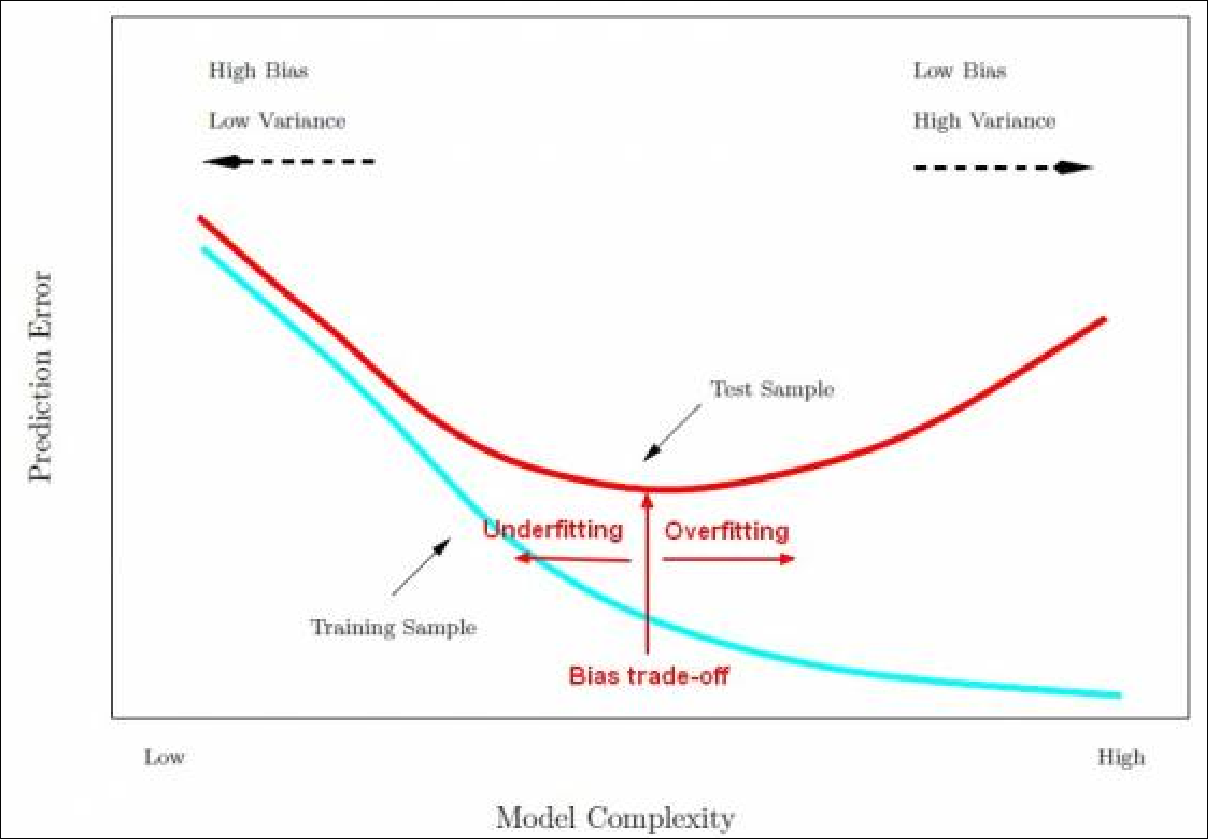
\includegraphics[width=0.5\textwidth]{img/2025-10-02-13-33-49.png}
\end{center}
Using decision trees, the model complexity corresponds to the depth of the tree. In a neural network it's the number of nodes.

\dfn{Overfitting}{

}

The problem is we don't know $ \mathcal{D} $, so we take two disjointed sets:
\begin{itemize}
\item \textbf{training set}: 
\item \textbf{validation set}: 
\end{itemize}

There are two ways to avoid overfitting:
\begin{itemize}
  \item \textbf{early stopping}: The top-down construction of the tree is stopped when the benefit to the precision of the model isn't relevant (based on the entropy gained)
  \item \textbf{post pruning}: the tree is first fully developped, then it's retroactivly 'pruned'
\end{itemize}

\subsection{Reduce-error post-pruning}
Uses the validation set to calculate the accuracy loss when removing subtrees. Notice how the model is still biased to the validation set, so a third set should be used to correctly assess the model's accuracy.

\section{Random Forests}
Instead of just one decision tree, why don't we use an ensamble of trees whose output is the weighted mean of all the outputs. Seen as the construction of a tree is completly determined by the set of training data and the features analyzed, we can use two different methods to differentiate trees in a random forest:
\begin{itemize}
\item \textbf{Bagging}:
\item \textbf{Feature randomness}:
\end{itemize}




% \end{document}
